\documentclass{standalone}
\usepackage{tikz}
\usetikzlibrary{patterns, positioning}


\begin{document}
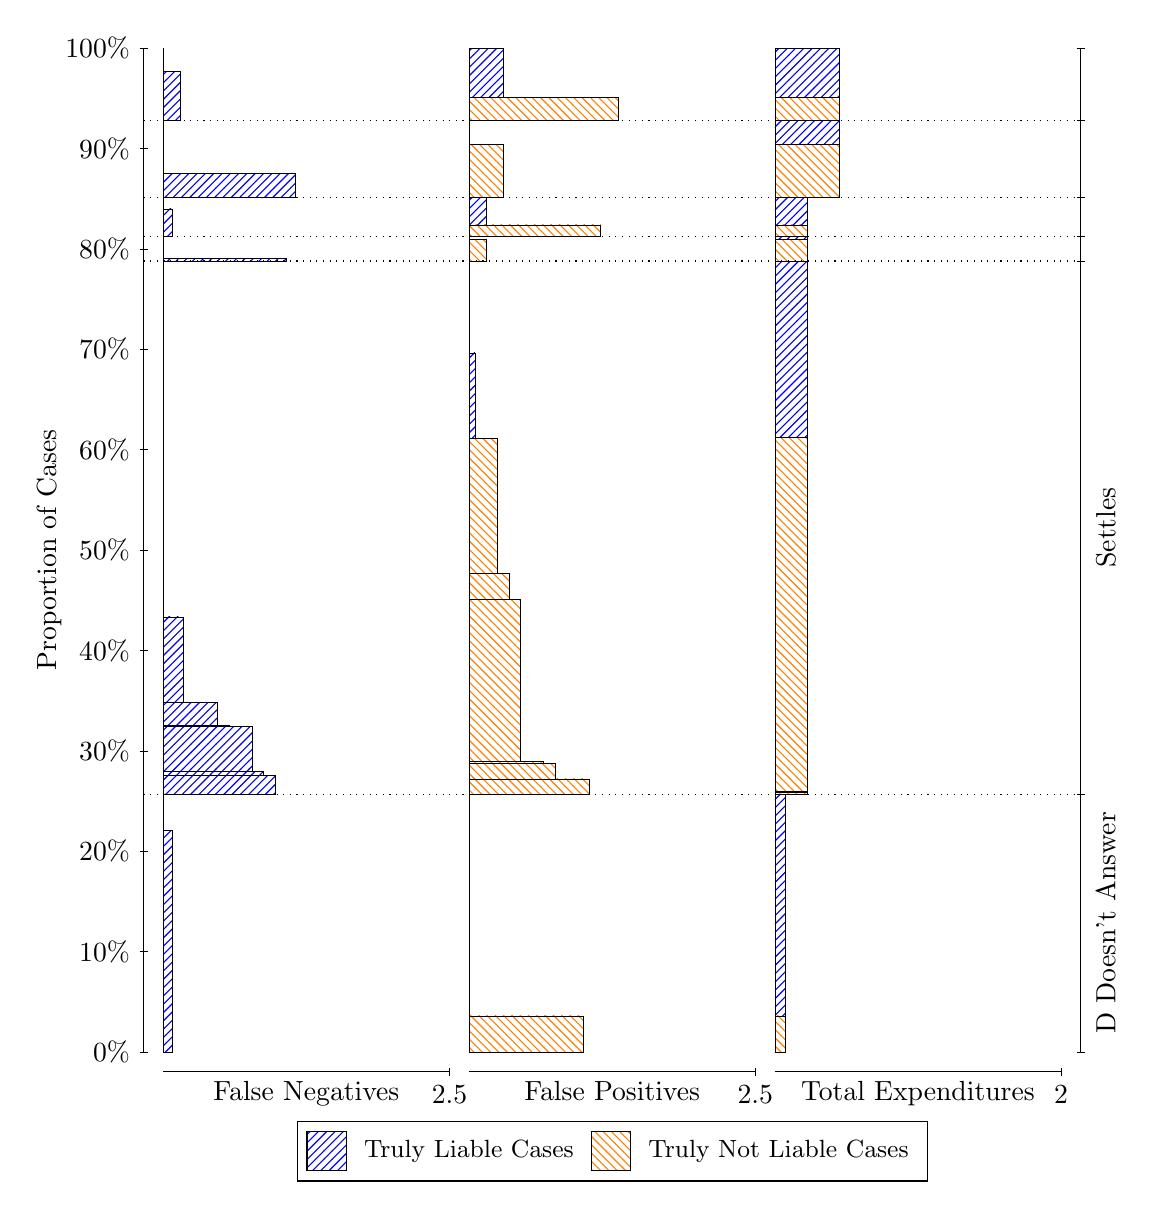
\begin{tikzpicture}
\draw[black, very thin] (1.5,1.75) -- (1.5,14.5);
\node[rotate=90, text=black, anchor=center] at (0.3, 8.125) {Proportion of Cases};
\draw[black, very thin] (1.45,1.75) -- (1.55,1.75);
\node[text=black, anchor=east] at (1.45, 1.75) {0\%};
\draw[black, very thin] (1.45,3.025) -- (1.55,3.025);
\node[text=black, anchor=east] at (1.45, 3.025) {10\%};
\draw[black, very thin] (1.45,4.3) -- (1.55,4.3);
\node[text=black, anchor=east] at (1.45, 4.3) {20\%};
\draw[black, very thin] (1.45,5.575) -- (1.55,5.575);
\node[text=black, anchor=east] at (1.45, 5.575) {30\%};
\draw[black, very thin] (1.45,6.85) -- (1.55,6.85);
\node[text=black, anchor=east] at (1.45, 6.85) {40\%};
\draw[black, very thin] (1.45,8.125) -- (1.55,8.125);
\node[text=black, anchor=east] at (1.45, 8.125) {50\%};
\draw[black, very thin] (1.45,9.4) -- (1.55,9.4);
\node[text=black, anchor=east] at (1.45, 9.4) {60\%};
\draw[black, very thin] (1.45,10.675) -- (1.55,10.675);
\node[text=black, anchor=east] at (1.45, 10.675) {70\%};
\draw[black, very thin] (1.45,11.95) -- (1.55,11.95);
\node[text=black, anchor=east] at (1.45, 11.95) {80\%};
\draw[black, very thin] (1.45,13.225) -- (1.55,13.225);
\node[text=black, anchor=east] at (1.45, 13.225) {90\%};
\draw[black, very thin] (1.45,14.5) -- (1.55,14.5);
\node[text=black, anchor=east] at (1.45, 14.5) {100\%};

\draw[black, very thin] (13.4,1.75) -- (13.4,14.5);
\draw[black, very thin] (13.35,1.75) -- (13.45,1.75);
\node[anchor=west] at (13.35, 1.75) {};
\draw[black, very thin] (13.35,5.0249) -- (13.45,5.0249);
\node[anchor=west] at (13.35, 5.0249) {};
\draw[black, very thin] (13.35,11.795) -- (13.45,11.795);
\node[anchor=west] at (13.35, 11.795) {};
\draw[black, very thin] (13.35,12.104) -- (13.45,12.104);
\node[anchor=west] at (13.35, 12.104) {};
\draw[black, very thin] (13.35,12.607) -- (13.45,12.607);
\node[anchor=west] at (13.35, 12.607) {};
\draw[black, very thin] (13.35,13.577) -- (13.45,13.577);
\node[anchor=west] at (13.35, 13.577) {};
\draw[black, very thin] (13.35,14.5) -- (13.45,14.5);
\node[anchor=west] at (13.35, 14.5) {};

\draw[black, very thin, pattern color=blue, pattern=north east lines] (1.75,1.75) rectangle (1.859,4.567);
\draw[black, very thin, pattern color=orange, pattern=north west lines] (1.75,4.567) rectangle (1.75,5.0249);
\draw[black, very thin, pattern color=blue, pattern=north east lines] (1.75,5.0249) rectangle (3.167,5.2662);
\draw[black, very thin, pattern color=blue, pattern=north east lines] (1.75,5.2662) rectangle (3.0217,5.3174);
\draw[black, very thin, pattern color=blue, pattern=north east lines] (1.75,5.3174) rectangle (2.8763,5.886);
\draw[black, very thin, pattern color=blue, pattern=north east lines] (1.75,5.886) rectangle (2.5857,5.899);
\draw[black, very thin, pattern color=blue, pattern=north east lines] (1.75,5.899) rectangle (2.4403,6.1908);
\draw[black, very thin, pattern color=blue, pattern=north east lines] (1.75,6.1908) rectangle (2.0043,7.2748);
\draw[black, very thin, pattern color=orange, pattern=north west lines] (1.75,7.2748) rectangle (1.75,11.795);
\draw[black, very thin, pattern color=blue, pattern=north east lines] (1.75,11.795) rectangle (3.3123,11.829);
\draw[black, very thin, pattern color=orange, pattern=north west lines] (1.75,11.829) rectangle (1.75,12.104);
\draw[black, very thin, pattern color=blue, pattern=north east lines] (1.75,12.104) rectangle (1.859,12.456);
\draw[black, very thin, pattern color=orange, pattern=north west lines] (1.75,12.456) rectangle (1.75,12.607);
\draw[black, very thin, pattern color=blue, pattern=north east lines] (1.75,12.607) rectangle (3.4213,12.904);
\draw[black, very thin, pattern color=orange, pattern=north west lines] (1.75,12.904) rectangle (1.75,13.577);
\draw[black, very thin, pattern color=blue, pattern=north east lines] (1.75,13.577) rectangle (1.968,14.203);
\draw[black, very thin, pattern color=orange, pattern=north west lines] (1.75,14.203) rectangle (1.75,14.5);
\draw[black, very thin, pattern color=orange, pattern=north west lines] (5.6333,1.75) rectangle (7.0867,2.2079);
\draw[black, very thin, pattern color=blue, pattern=north east lines] (5.6333,2.2079) rectangle (5.6333,5.0249);
\draw[black, very thin, pattern color=orange, pattern=north west lines] (5.6333,5.0249) rectangle (7.1593,5.2193);
\draw[black, very thin, pattern color=orange, pattern=north west lines] (5.6333,5.2193) rectangle (6.7233,5.4168);
\draw[black, very thin, pattern color=orange, pattern=north west lines] (5.6333,5.4168) rectangle (6.578,5.4415);
\draw[black, very thin, pattern color=orange, pattern=north west lines] (5.6333,5.4415) rectangle (6.2873,7.4935);
\draw[black, very thin, pattern color=orange, pattern=north west lines] (5.6333,7.4935) rectangle (6.142,7.8293);
\draw[black, very thin, pattern color=orange, pattern=north west lines] (5.6333,7.8293) rectangle (5.9967,9.545);
\draw[black, very thin, pattern color=blue, pattern=north east lines] (5.6333,9.545) rectangle (5.706,10.629);
\draw[black, very thin, pattern color=blue, pattern=north east lines] (5.6333,10.629) rectangle (5.6333,11.795);
\draw[black, very thin, pattern color=orange, pattern=north west lines] (5.6333,11.795) rectangle (5.8513,12.07);
\draw[black, very thin, pattern color=blue, pattern=north east lines] (5.6333,12.07) rectangle (5.6333,12.104);
\draw[black, very thin, pattern color=orange, pattern=north west lines] (5.6333,12.104) rectangle (7.3047,12.255);
\draw[black, very thin, pattern color=blue, pattern=north east lines] (5.6333,12.255) rectangle (5.8513,12.607);
\draw[black, very thin, pattern color=orange, pattern=north west lines] (5.6333,12.607) rectangle (6.0693,13.28);
\draw[black, very thin, pattern color=blue, pattern=north east lines] (5.6333,13.28) rectangle (5.6333,13.577);
\draw[black, very thin, pattern color=orange, pattern=north west lines] (5.6333,13.577) rectangle (7.5227,13.875);
\draw[black, very thin, pattern color=blue, pattern=north east lines] (5.6333,13.875) rectangle (6.0693,14.5);
\draw[black, very thin, pattern color=orange, pattern=north west lines] (9.5167,1.75) rectangle (9.6529,2.2079);
\draw[black, very thin, pattern color=blue, pattern=north east lines] (9.5167,2.2079) rectangle (9.6529,5.0249);
\draw[black, very thin, pattern color=orange, pattern=north west lines] (9.5167,5.0249) rectangle (9.9254,5.0496);
\draw[black, very thin, pattern color=blue, pattern=north east lines] (9.5167,5.0496) rectangle (9.9254,5.0626);
\draw[black, very thin, pattern color=orange, pattern=north west lines] (9.5167,5.0626) rectangle (9.9254,9.558);
\draw[black, very thin, pattern color=blue, pattern=north east lines] (9.5167,9.558) rectangle (9.9254,11.795);
\draw[black, very thin, pattern color=orange, pattern=north west lines] (9.5167,11.795) rectangle (9.9254,12.07);
\draw[black, very thin, pattern color=blue, pattern=north east lines] (9.5167,12.07) rectangle (9.9254,12.104);
\draw[black, very thin, pattern color=orange, pattern=north west lines] (9.5167,12.104) rectangle (9.9254,12.255);
\draw[black, very thin, pattern color=blue, pattern=north east lines] (9.5167,12.255) rectangle (9.9254,12.607);
\draw[black, very thin, pattern color=orange, pattern=north west lines] (9.5167,12.607) rectangle (10.334,13.28);
\draw[black, very thin, pattern color=blue, pattern=north east lines] (9.5167,13.28) rectangle (10.334,13.577);
\draw[black, very thin, pattern color=orange, pattern=north west lines] (9.5167,13.577) rectangle (10.334,13.875);
\draw[black, very thin, pattern color=blue, pattern=north east lines] (9.5167,13.875) rectangle (10.334,14.5);
\draw[black, dotted] (1.5,5.0249) -- (13.4,5.0249);
\draw[black, dotted] (1.5,11.795) -- (13.4,11.795);
\draw[black, dotted] (1.5,12.104) -- (13.4,12.104);
\draw[black, dotted] (1.5,12.607) -- (13.4,12.607);
\draw[black, dotted] (1.5,13.577) -- (13.4,13.577);
\draw[black, very thin] (1.75,1.5) -- (5.3833,1.5);
\node[text=black, anchor=north] at (3.5667, 1.5) {False Negatives};
\draw[black, very thin] (5.3833,1.45) -- (5.3833,1.55);
\node[text=black, anchor=north] at (5.3833, 1.45) {2.5};

\draw[black, very thin] (5.6333,1.5) -- (9.2667,1.5);
\node[text=black, anchor=north] at (7.45, 1.5) {False Positives};
\draw[black, very thin] (9.2667,1.45) -- (9.2667,1.55);
\node[text=black, anchor=north] at (9.2667, 1.45) {2.5};

\draw[black, very thin] (9.5167,1.5) -- (13.15,1.5);
\node[text=black, anchor=north] at (11.333, 1.5) {Total Expenditures};
\draw[black, very thin] (13.15,1.45) -- (13.15,1.55);
\node[text=black, anchor=north] at (13.15, 1.45) {2};

\node[text=black, centered, rotate=90] at (13.72, 3.3874) {D Doesn't Answer};
\node[text=black, centered, rotate=90] at (13.72, 8.4099) {Settles};





\draw (7.449999999999999,1.5) node[draw=none] (baseCoordinate) {};
\begin{scope}[align=center]
        \matrix[scale=0.5, draw=black, below=0.5cm of baseCoordinate, nodes={draw}, column sep=0.1cm]{
            \node[rectangle, draw, minimum width=0.5cm, minimum height=0.5cm, pattern color=blue, pattern=north east lines] {}; &
            \node[draw=none, font=\small, text=black] (B) {Truly Liable Cases}; &
            \node[rectangle, draw, minimum width=0.5cm, minimum height=0.5cm, pattern color=orange, pattern=north west lines] {}; &
            \node[draw=none, font=\small, text=black] (B) {Truly Not Liable Cases}; \\
            };
\end{scope}

\end{tikzpicture}
\end{document}